%%%%%%%%%%%%%%%%%%%%%%%%%%%%%%%%%%%%%%%%%%%%%%%%%%%%%%%%%%%%%%%%%%%%%%%%%%%%%%%
%
% Tommy P. Keane
% Master of Science Thesis
% Department of Electrical and Microelectronic Engineering
% Rochester Institute of Technology
%
% April 2011
%
%
%
% Funded By: Lenel Systems Inc., A UTC Fire & Security Corporation
%
% Algorithm Intellectual Property Owned By: Lenel Systems Inc.
%
%
% http://www.tommypkeane.com
%
%%%%%%%%%%%%%%%%%%%%%%%%%%%%%%%%%%%%%%%%%%%%%%%%%%%%%%%%%%%%%%%%%%%%%%%%%%%%%%%

%%%%%%%%%%%%%%%%%%%%%%%%%%%%%%%%%%%%%%%%%%%%%%%%%%%%%%%%%%%%%%%%%%%%%%%%%%%%%%%
%
% CHAPTER 2
%
% SECTION 5: Camera Geometry
%
%%%%%%%%%%%%%%%%%%%%%%%%%%%%%%%%%%%%%%%%%%%%%%%%%%%%%%%%%%%%%%%%%%%%%%%%%%%%%%%


%%%%%%%%%%%%%%%%%%%%%%%%%%%%%%%%%%%%%%%%%%%%%%%%%%%%%%%%%%%%%%%%%%%%%%%%%%%%%%%
% BEGIN DOCUMENT

Sections 2.3 and 2.4 have presented the mathematics and concepts required for building the mutual information metric and applying it to digital images. The final major concept to understand in the theoretical development and motivation is how multiple views of a single scene can be related mathematically. Also, this section presents the major obstacles in multi-view geometry, specifically parallax differences and occlusions, as a mathematical model for relating views is only as useful as its constraints and assumptions when applying it to real-world scenarios.

As the discussion has been already laid out, there are three distinct coordinate systems present in the mathematics discussed here. There are the scene coordinates: the 3-dimensional spatial world with time; the camera (view) coordinates (the digital video): a 2-dimensional spatial domain with a third dimension for color and a fourth dimension for time; and the frame coordinates: the 2-dimensional, plus the third dimension for color, image extracted from the video. The camera view projects the real-world scene onto the 2-D spatial domain of the camera plane while preserving the time dimension (albeit sampled and quantized in all of these dimension), and the frame is an instance of the time dimension of the camera. There is no quantization when looking at the frame versus the video, and it is not conceptually useful to think of it as sampling, it is an extraction. Video compression concerns will be ignored in this development though they play a role in the success of the algorithm, but simplistically they can be thought of as  more quantization and interpolation. Similar to what will be discussed in Chapter 6's review of potential future applications in motion tracking or estimation, multiple frames could be incorporated to build a more accurate metric and alleviate many of the concerns and obstacles of registering multiple views.

Understanding camera geometry is most easily understood by modeling the digital camera as a spatial projection system with a pinhole/point aperture \cite{Hartley2003}. Extending all of the following to realistic apertures would mostly just modify image spatial resolution and essentially creates a blurring effect on the results. Including this would only complicate the discussion as ray geometry would have to be abandoned for wavefront physics. So, again, the camera is thought of as a system that takes the light reflected and refracted off of the objects in the scene, allows it to pass through the point aperture (modeled as rays), and captures the light rays at the sample locations on the CCD array (which again has the Bayer filter in the case of color imagery). Following this understanding of ray optics there will be several main components of the camera model: real-world points, the point/conic/plane at infinity (the vanishing point), the image plane, and the camera center (a point). This model for a single camera is shown in Figure \ref{CameraModel}.

\begin{figure}[h]
\centering
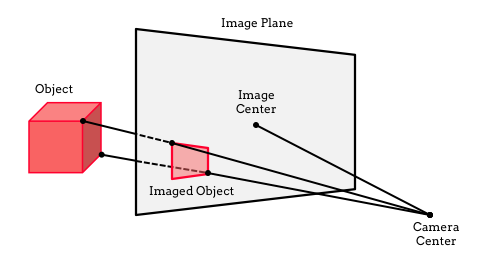
\includegraphics[width=.9\textwidth]{CameraModel}
\caption{Projective Camera System Model}
\label{CameraModel}
\end{figure}


Again, it is clear in this model that there are the 3-D objects in the scene that become projected through the camera aperture (not shown for simplification) onto the camera's image plane as a 2-D imaged object. As the camera center moves in relation to the object in the scene, the projection of the object will clearly change. Looking at Figure \ref{CameraModel}, the idea in this algorithm's applicable scenarios is that the object (the scene) and the cameras (the views) will remain stationary but these other cameras viewing the same object will have distinct projections of the scene onto their image planes. In this model the object is highly symmetric so there will be many views that seem identical but real-world objects are not typically this symmetric; although they do have typically rigid shapes with relatively smooth textures, \ie{ }large areas of low entropy. Clearly for multiple views, the closer the camera centers are, the more similar the views will be. If the scene has many objects and a lot of 3-dimensional spatial variation, then it will require less and less distance between camera centers for the views to change significantly. Yet modeling a general scene as having a significant but not extensive amount of 3-dimensional variation can fall back to the discussion on regional PMFs, where the overlapping regions in the views (the sections of the images observing the same objects in the scene) will be similar enough in intensity or projected scene content that their PMFs should have a higher mutual information than any other combination of regions (in a scene with modest entropy).

But, there are more complex scenarios (that are unfortunately more realistic) where this argument does not seem to follow as directly as it just did. Figure \ref{CameraOcclusion} shows a scene with two objects viewed by two cameras, resulting in the two distinct projections, but now there is clear variation in the amounts of parallax and occlusion in each view's frame.


\begin{figure}[h]
\centering
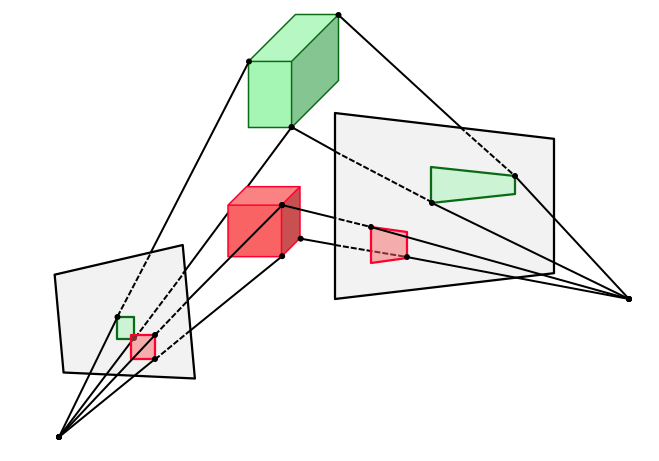
\includegraphics[width=.9\textwidth]{CameraOcclusion}
\caption{Multiple Projective Cameras Model}
\label{CameraOcclusion}
\end{figure}

\noindent The camera on the left's image suffers from occlusion where the red block is covering a corner of the green block, as also indicated by the paths of the rays. There is also the effect of parallax, wherein with each view the distance between projected objects in the images varies based on the camera's distance to the objects in the scene. The red and green blocks appear very close together spatially in the left view but are spaced far apart in the right view. Occlusion and parallax are not just characteristics of the views, they are characteristic of the entire scenario: the scene, its objects, and the views. This model, however, is an extreme case as a panorama would not be easily generated or viewable in a 2-D display given these views. Also, the objects imaged are essentially being imaged orthogonally by the cameras and so without some strong symmetry in the objects there would be no correspondence between the views; and that symmetry would be a false registration, just as in the case of registering two non-overlapping views of an extremely low entropy scene (constant colored or textured flat surface). The registration could seem accurate but it would be trivial and incorrect, which would be discernible as soon as an object began a non-symmetrical motion (that is symmetry between the views).

So ultimately what is applicable to this algorithm that needs to be understood about camera geometry? Projection is the main thrust of this discussion, even though multi-view geometry is an extremely rich and interesting topic, because the goal of this algorithm is to generate convincing panoramas of realistic scenes, automatically. Views like those modeled in Figure \ref{CameraOcclusion} are certainly relatable through epipolar constraints and use of a Fundamental matrix \cite{Hartley2003}, but they would not produce a 2-D panorama. Clearly there must be some initial restriction, in the basic theory, where camera centers are not at angles of rotation much beyond 45\textsuperscript{o} to one another with respect to their views. Realistically, \ie{ }in practice, this is a general and typical scenario as cameras will be placed along typically rectangular structures such as buildings and fence lines or in hallways. Yet even in these scenarios, there will be significant occurrences of occlusion, and differences in occlusion between views stemming from parallax discrepancies. If an object is occluded in one view and not the other, such as the bottom corner of the green box, any point-to-point correspondence algorithm that considered that corner of the box a feature, would find it in one view but not the other, thus that correspondence would not and could not be used in registration. The more complex the scene is, such as irregular shaped objects and large variations in 3-dimensional arrangements, there will be many points existing in one view that do not exist in the other. This discussion will be expanded in the next chapter, but this is the foundational motivation for designing the WFMI algorithm as a region-based correspondence rather than a point-based correspondence algorithm. And limiting it to rigid contiguous regions maintains the structure of the scene. Point-to-point correspondence can allow for more realistic deformations, but it can also allow for very unrealistic deformations. Given that that corner of the green box was found in one view and not the other, it could be searched for in the second view and accidentally corresponded to some other point in the scene. Using that relationship to develop the homography or transformation between the views \cite{Hartley2003} can produce extreme inaccuracy.

The next chapter will discuss the details of the implementation of the algorithm based on these theories, but it is important to understand that occlusion and parallax are extremely difficult to model but occur extremely often in realistic scenarios. With no known relationship between camera locations, the WFMI algorithm took this knowledge of multi-view geometry and its constraints to assume that even though there will not be a full set of points in an overlap region that can be corresponded, the structure and arrangement of objects will be there and that's what should be searched for. This is why it is a region based algorithm, as it compares scenes based on the structure and arrangement of the objects, not the exact location of the objects. That is also why it is so successful despite only searching for an affine relationship between views more accurately relatable by a projective homography or a Fundamental matrix.

%%%%%%%%%%%%%%%%%%%%%%%%%%%%%%%%%%%%%%%%%%%%%%%%%%%%%%%%%%%%%%%%%%%%%%%%%%%%%%%
% END OF DOCUMENT

